\chapter{Experimental Apparatus}
\label{chap:apparatus}

\graphicspath{{2_Experimental_Apparatus/Figures/}}

\section{The Large Hadron Collider}
\label{sec:large_had_collider}

The Large Hadron Collider (LHC), located near Geneva, Switzerland, is a super-conducting circular particle accelerator, 
consisting of a 27-kilometer ring of superconducting magnets. For the majority of the time, protons are used as the accelerated
particles, but in addition to protons, Xe and Pb ions are also used for heavy ion studies. For the context of this thesis, data
from only the proton collisions are being considered.

Two sets of proton bunches travel along the circular tunnel in opposite directions, being accelerated to near the speed of light,
then collide at the experiment sites. The four large experiments located at the LHC ring are CMS, ATLAS, LHCb and ALICE. CMS and ATLAS
are multi-purpose detectors, while LHCb focuses on heavy hadron physics, and ALICE focuses on heavy ion physics. The center-of-mass energy 
for the proton-proton collision for Run II is 13 TeV. This energy is further increased to 13.6 TeV in 
more recent runs of the LHC, corresponding to Run III. 

Protons are accelerated through a chain of accelerators before they reach LHC, which is shown in Fig.~\ref{fig:lhc_diagram}.
Each machine boosts the energy of protons before injecting it into the next machine in the sequence. Linear Accelerator 4 (LINAC4)
is the source of protons, accelerating $H^{-}$ ions to 160 MeV to prepare them to enter the Proton Synchotron Booster (PSB). During the injection
to PSB, the two ions are stripped from the $H^{-}$ ions, leaving only the protons. These protons are accelerated to 2 GeV for injection to Proton 
Synchotron (PS), which increases the beam energy to 26 GeV. The proton beam is then sent to Super Proton Synchotron (SPS), where it is accelerated
to an energy of 450 GeV. Finally, the proton beam is transferred to the two beam pipes of the LHC. Here, it takes 20 minutes for the protons to reach
their maximum energy of 6.5 TeV. 

\begin{figure}[htb]
    \begin{minipage}[t]{\linewidth}\centering
        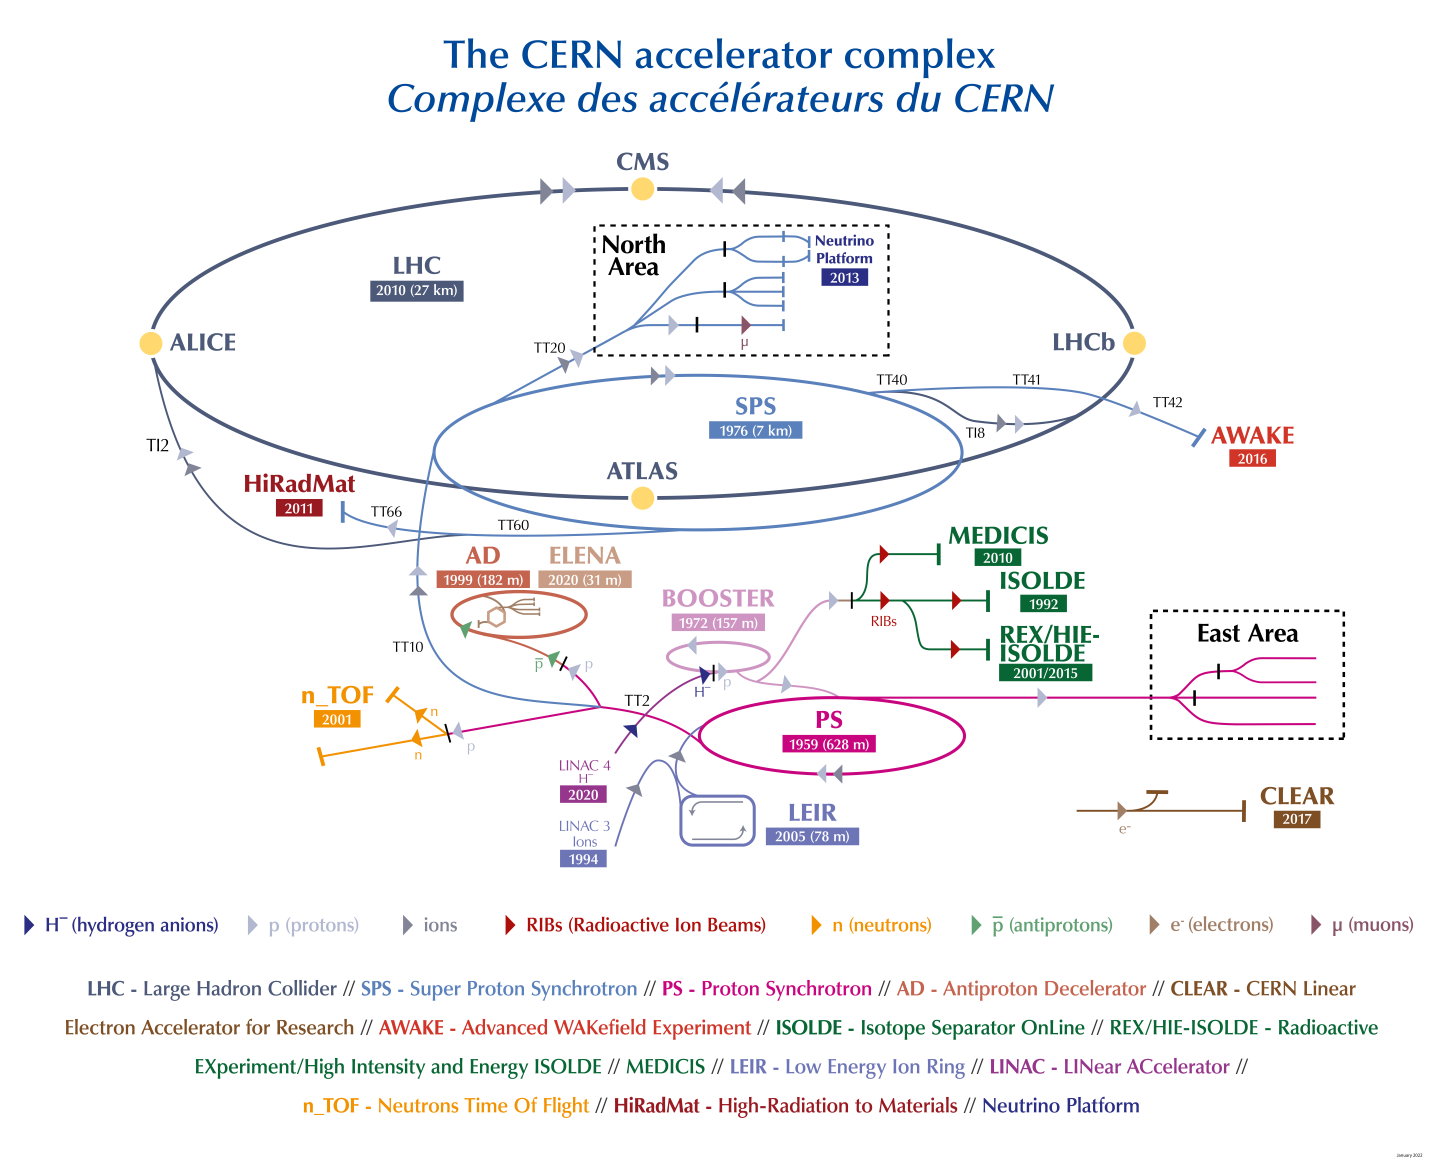
\includegraphics[width=15cm]{lhc_complex.png}
    \end{minipage}
    \caption{Diagram of the CERN accelerator complex, showing the LHC and the chain of other accelerator rings. 
    Each ring boosts the energy of accelerated particles before injecting it into the next ring in the sequence.
    The diagram is taken from \cite{LHCAcceleratorComplex}.}
    \label{fig:lhc_diagram}
\end{figure}

The LHC had a successful Run I between 2010 and 2013, where the center-of-mass energy for proton-proton collisions was 8 TeV. This first run was marked 
by the discovery of the Higgs boson by ATLAS and CMS experiments in 2012. After a long shutdown, the center-of-mass energy was increased to 13 TeV, and the LHC
operated from 2016 to 2018 for Run II data taking. During Run II, the instantenous luminosity was about $1 \times 10^{34} \ cm^{-2} s^{-1}$, corresponding to around 
25 proton-proton collisions per bunch crossing. The integrated luminosity corresponding to Run II data taken by the CMS experiment is measured to be 137 $fb^{-1}$, 
with 1.6\% overall uncertainty \cite{lumi:2018,lumi:2017,lumi:2016}.

\section{The CMS Detector}

The CMS detector is a multi-purpose detector, designed trigger on \cite{cms:l1_paper,cms:hlt_paper} and detect muons, electrons, photons, charged and 
neutral hadrons \cite{cms:elepho_paper,cms:muon_paper,cms:vertex_paper}. To be able to identify this wide range of particles, the CMS detector uses a combination of signals from different sub-detectors. These signals
are then used in the Particle-Flow (PF) algorithm to reconstruct the particles in the event. The sub-detectors in the CMS detector are:

\begin{itemize}
    \item Tracking system
    \item Electromagnetic calorimeter (ECAL)
    \item Hadron calorimeter (HCAL)
    \item Muon system
\end{itemize}

CMS detector also uses a two-level trigger system \cite{cms:l1_paper,cms:hlt_paper}, to make physics-based decisions on the data being saved to disk, 
therefore reducing the output rate. In the following sub-sections, the functionality of these subsystems and the overall design of the CMS detector are discussed.

\subsection{Overall Layout}

The CMS detector has an overall length of 28.7 meters, and weighs 14000 tonnes. The cylindrical detector
has a diameter of 15 meters, as shown in Fig.~\ref{fig:cms_overall_diagram}. The CMS detector has a superconducting solenoid,
which has an internal diameter of 7 meters, and creates a magnetic field of 3.8 T. This magnetic field curves the charged particles
as they pass through the detector, hence enabling the measurement of their momentum from the radius of curvature of their tracks.


\begin{figure}
    \begin{minipage}[t]{\linewidth}\centering
        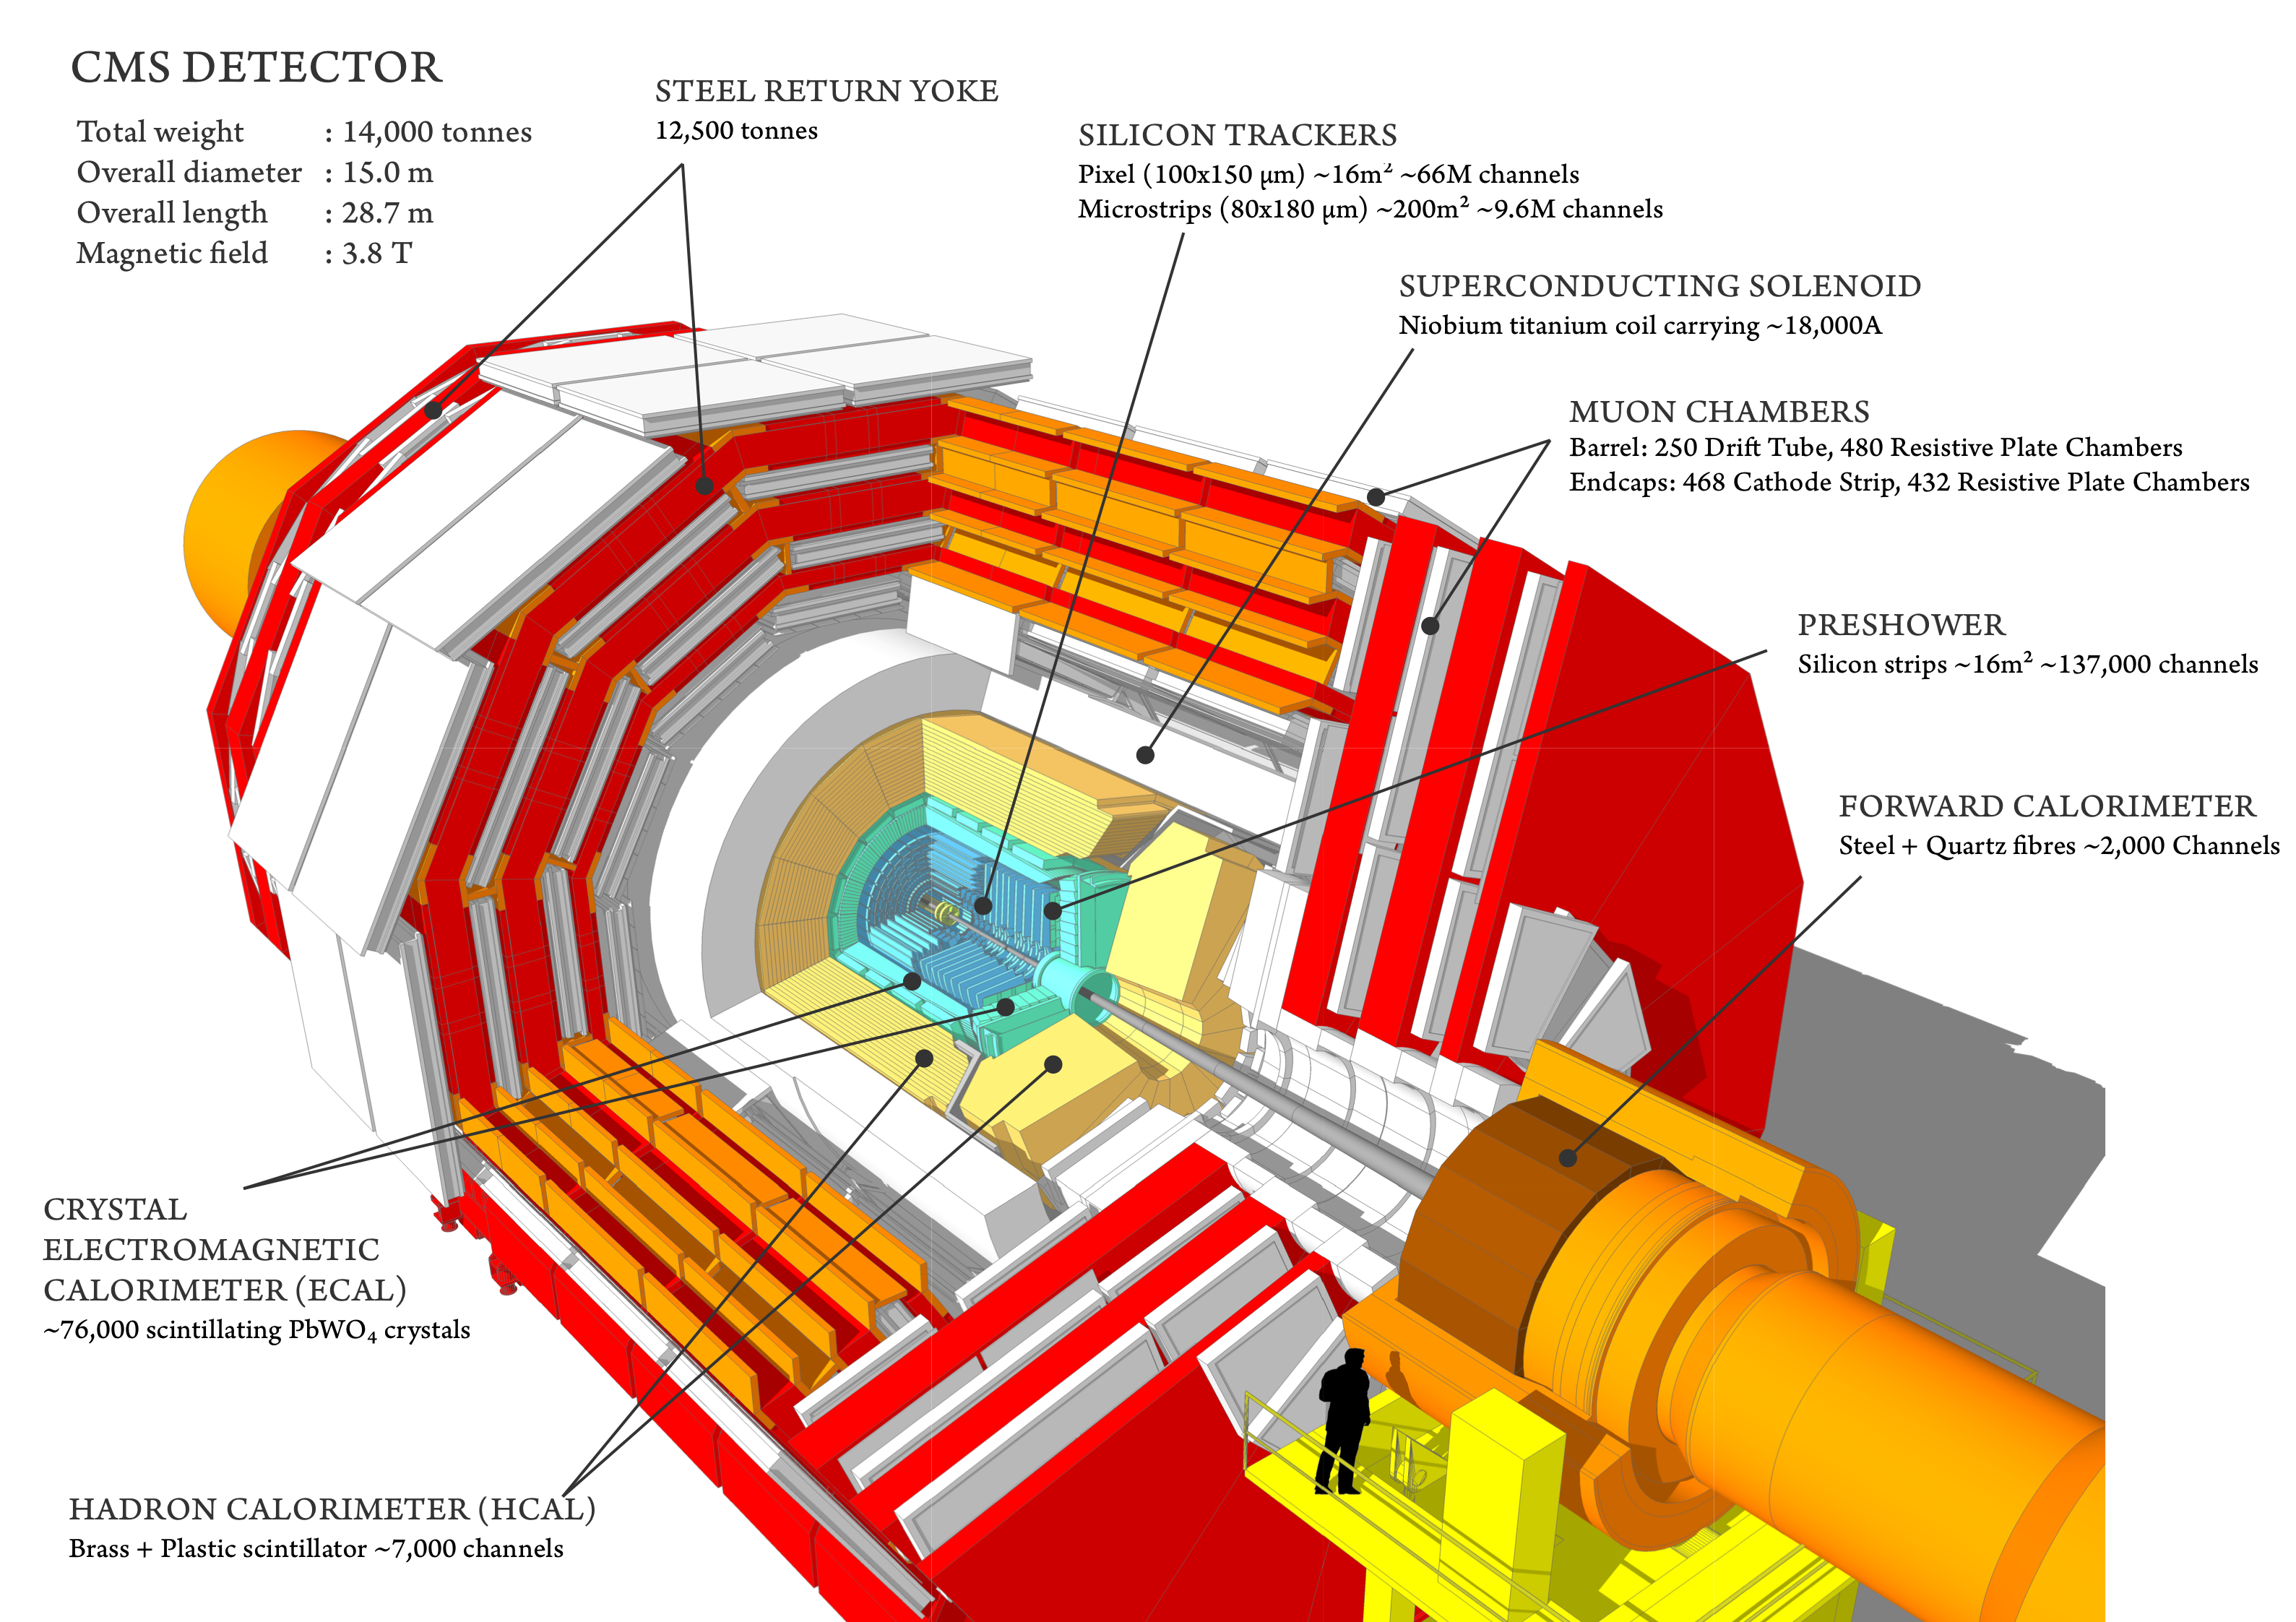
\includegraphics[width=15cm]{cms_detector.png}
    \end{minipage}
    \caption{Sectional view of the CMS detector. The LHC beams travel in opposite directions 
    along the central axis of the CMS cylinder colliding in the middle of the CMS detector \cite{detector:cms_overall}.}
    \label{fig:cms_overall_diagram}
\end{figure}

Within the solenoid volume are a silicon pixel and strip tracker, a lead tungstate crystal electromagnetic calorimeter (ECAL), 
and a brass and scintillator hadron calorimeter (HCAL), each composed of a barrel and two endcap sections. Forward calorimeters
are installed in the high psuedo-rapidity range to extend the coverage of the detector. Outside of the solenoid volume,
a muon detection system is installed, where muons are measured in gas-ionization detectors embedded in the steel flux-return yoke.

In the CMS detector, the right-handed coordinate system is used. The x-axis points to the center of the LHC ring, the y-axis points up, 
and the z-axis point along the beam in the counter-clockwise direction. Due to the cylindrical symmetry of the detector geometry, the angular
coordinates of $\eta$ and $\phi$ are often used to describe event kinematics. $\phi$ is the azimuthal angle, defined to be 0 along the x-axis,
and $\frac{\pi}{2}$ along the y-axis. $\eta$ is the psuedo-rapitiy, which depends on the angle from the z-axis, $\theta$, with the following
equation: $\eta = -\ln[{\tan({\frac{1}{\theta}})}]$. This way, $\eta$ equals to 0 along the z-axis, directly perpendicular to the beam-axis,
and $|\eta| \rightarrow \infty$ as the $\theta \rightarrow \frac{\pi}{2}$, i.e. perpendicular to the beam axis. Most detector coverage
extends to until $|\eta| = 5$. 

\subsection{Tracking System}

The innermost layer of the CMS detector is the tracking system. This tracking system consists of a silicon pixel detector and a silicon strip detector, 
referred to as the inner tracker and the outer tracker, respectively. Both are used to reconstruct tracks of charged particles, under the influence of
the 3.8 T magnetic field generated by the solenoid. The inner pixel detector has higher granularity, therefore it can reconstruct tracks more accurately near
the beam pipe, where the track density is higher.

Tracks of charged particles are crucial objects for CMS, because they allow measuring the momenta and the electrical charges of particles. These particles include
electrons, muons, taus and charged hadrons. The identification of tracks also allow to reconstruct the proton-proton collision vertices in the event. This enables
the identification of the primary vertex in the event with the highest sum of $p_{T,track}^{2}$. Thus, the rest of the vertices can be identified as pile-up (PU),
and charged particles from these PU vertices can be rejected in object reconstruction. Track reconstruction also allows to identify b-quarks by identifying displaced
vertices. 

The CMS inner tracker was upgraded during the year-end technical stop of the LHC in 2016/2017, referred to as the Phase-1 upgrade \cite{cms:tracker_upgrade},
in order to handle the instantaneous luminosity that exceeds the previously designed maximum value of $1 \times 10^{34} \ cm^{-2} s^{-1}$. Utilizing the new 
beam pipe with smaller radius installed during the LHC Long Shutdown 1 (LS1), the Phase-1 pixel detector sits closer to the beam center, with 4 barrel layers 
(L1-L4) at radii of 29, 68, 109, and 160 mm, compared to the original three layers at 44, 73, and 102 mm. There is also an additional endcap disk on each end 
closer to the collision point. Therefore, there are now three disks at each end with distances of 291, 396, and 516 mm from the center of the detector, compared 
to the original three layers at 345 and 465 mm. This new layout is optimized to have 4-hit coverage for tracks within $|\eta| < 2.5$. The original and the upgraded
pixel detector layouts are shown in Fig.~\ref{fig:cms_tracker_upgrade}.

\begin{figure}
    \begin{minipage}[t]{\linewidth}\centering
        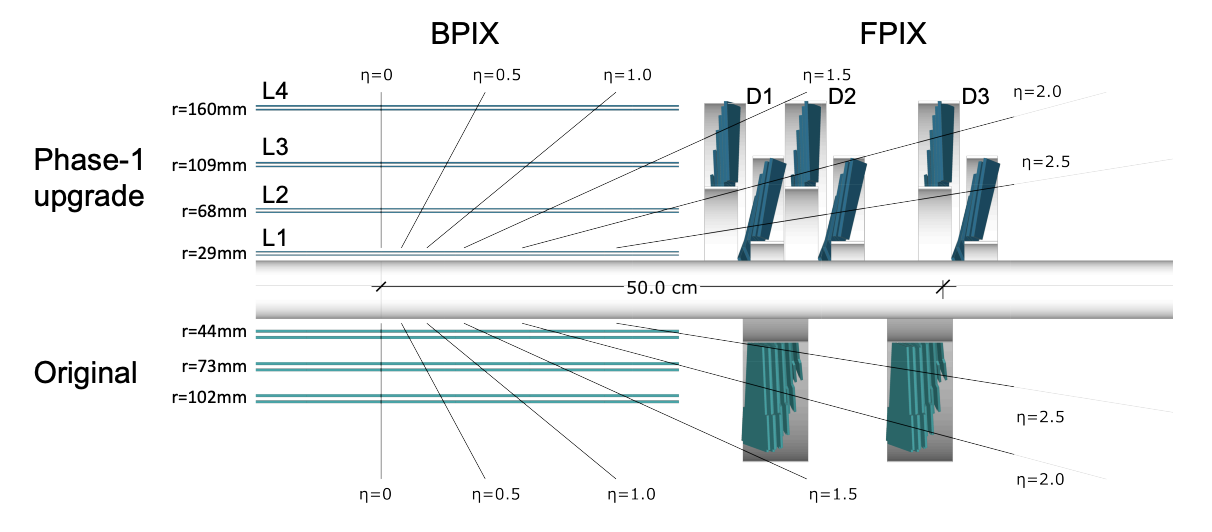
\includegraphics[width=15cm]{inner_tracker_layout.png}
    \end{minipage}
    \caption{Comparison of the layouts between the original pixel detector (bottom) and the Phase-1 upgraded pixel detector (top) \cite{cms:tracker_upgrade}.}
    \label{fig:cms_tracker_upgrade}
\end{figure}

Outside of the pixel detector, the silicon strip tracker is installed, which consists of three subsystems:  the Tracker Inner Barrel and Disks (TIB/TID), 
the Tracker Outer Barrel (TOB), and the the Tracker EndCaps (TEC). Their radii range from 20 cm to 116 cm and are up to 282 cm away from the detector center 
in the z direction. The layout of the silicon strip tracker, together with the 2016 version of the pixel detector, is shown in Fig.~\ref{fig:cms_full_tracker_layout}.

\begin{figure}
    \begin{minipage}[t]{\linewidth}\centering
        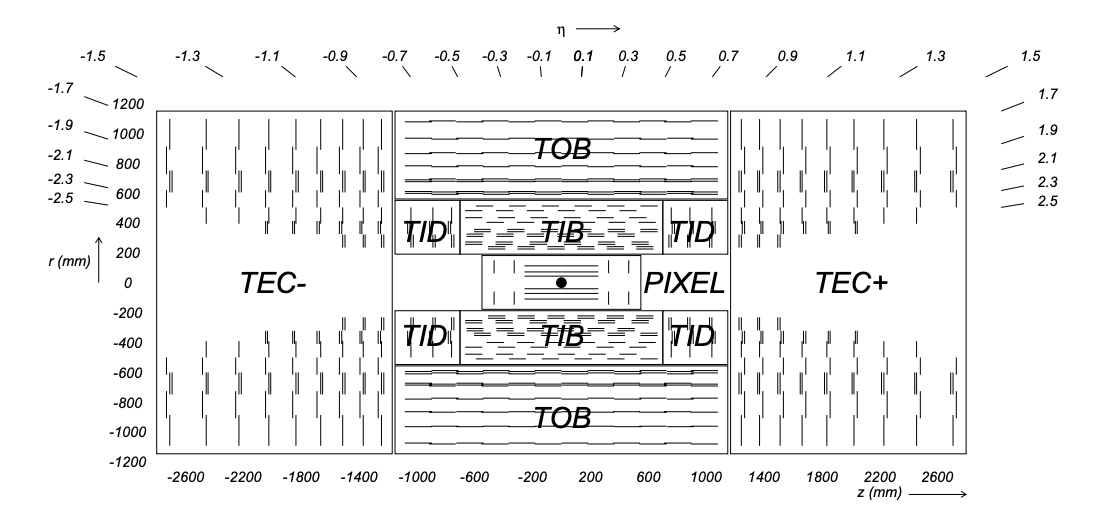
\includegraphics[width=15cm]{full_tracker_layout.png}
    \end{minipage}
    \caption{Schematic cross section through the CMS tracker. Notice that the pixel detector is shown as the 2016 version.
    The image is taken from \cite{cms:cms_experiment}.}
    \label{fig:cms_full_tracker_layout}
\end{figure}

\subsection{Electromagnetic Calorimeter}

The electromagnetic calorimeter (ECAL) is installed on the second layer of the detector, outside the inner and outer tracking systems. It is made of
61200 lead tungstate ($PbWO_{4}$) crystals mounted in the barrel (EB), and 7324 of those crystals in each of the 2 endcaps (EE). The $PbWO_{4}$ crystals make
a radiation-resistent high-granularity calorimeter, due to it's high density and short radiation length. The EB section covers the psuedo-rapidity range
of $|\eta| < 1.479$, and the two EE sections cover $1.479 < |\eta| < 3.0$.

The energy of particles, primarily electrons and photons, are measured through the scintillation effect. Photons emitted from the scintillation are 
collected by the avalanche photodiodes (APD) in the barrel and vacuum phototriodes (VPT) in the EE. Two pre-shower detectors are placed on the inner side
of the EEs, which helps to distinguish high-energy photons from pions, which can decay into a pair of closeby low-energy photons. The preshower is a sampling 
calorimeter made of two planes on each end. Each plane has a layer of lead radiators to produce electromagnetic showers from incoming photons and electrons, 
and a silicon strip detector to mea- sure the energy and shower profile. The silicon strips are placed with a width of 2 mm, and are oriented in perpendicular 
directions between two layers, giving a much finer granularity than EE and EB. 

The crystals in the barrel section are contained by 1 mm wall of aluminum, which constitues a submodule. 400 or 500 submodules are assembled into a module, 
and every four of each constitute a supermodule. The crystals in the EE are organized in units of identically shaped $5 \times 5$ crystals called supercrystals. 
Each EE is divided into two halves (Dees). The structure of the ECAL is shown in Fig.~\ref{fig:ecal_layout}.

\begin{figure}
    \begin{minipage}[t]{\linewidth}\centering
        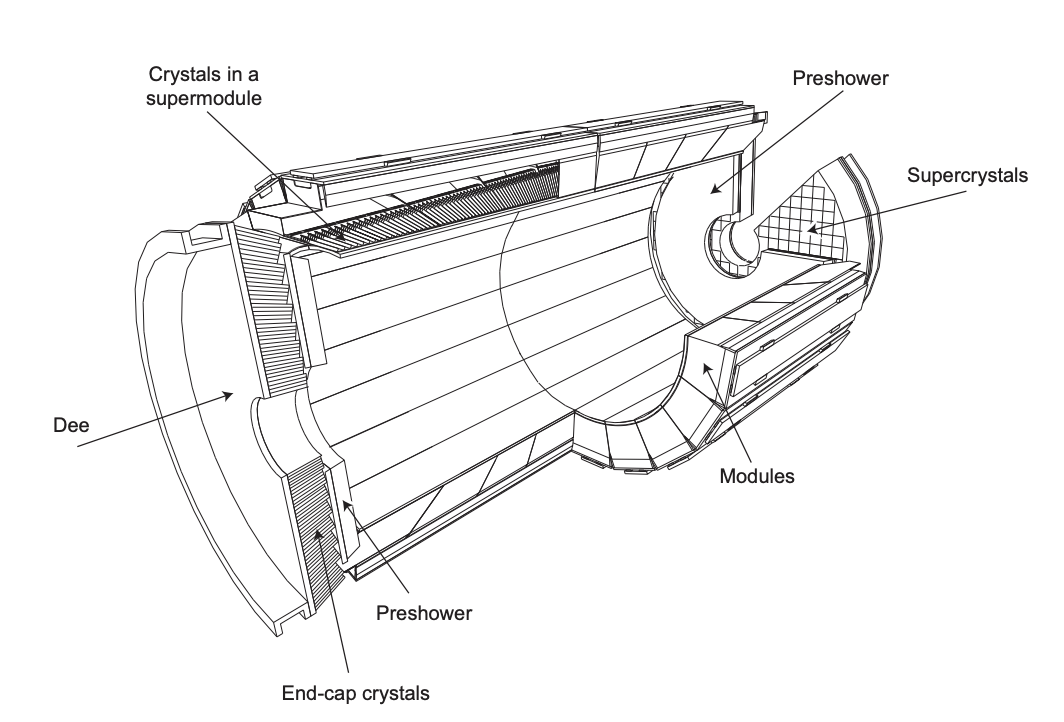
\includegraphics[width=15cm]{ecal_layout.png}
    \end{minipage}
    \caption{Layout of the CMS electromagnetic calorimeter showing the arrangement of crystal
    modules, supermodules and endcaps, with the preshower in front \cite{cms:cms_experiment}.}
    \label{fig:ecal_layout}
\end{figure}


\subsection{Hadron Calorimeter}
\label{subsec:hcal}

The hadron calorimeter (HCAL) is designed to measure the energy of hadrons, which is specifically important for reconstructing and measuring the energy of
hadron jets. The HCAL is composed of several parts: 

\begin{itemize}
    \item A barrel part (HB), which sits between the ECAL and the magnet coil, covering the range of $|\eta| < 1.3$. 
    \item An endcap part (HE), covering the range of $1.3 < |\eta|< 3$.
    \item Forward hadron calorimeters (HF), which are placed close to the beam pipe to capture outgoing particles with small angles, covering up to $|\eta| < 5$.
\end{itemize}

Due to the limited space between the ECAL and the magnet coils, additional hadron calorimeters (HO) are placed outside of the magnet coils to help 
contain hadron showers. The layout of the HCAL detector is shown in Fig.~\ref{fig:hcal_layout}.

The majority of HCAL is a sampling calorimeter made of alternating absorbing layers of brass and plastic scintillating layers. 
The forward calorimeter HF utilizes a different design, which consists of a steel absorber and quartz fibers that generate Cherenkov light, 
in order to operate in a much harsher radiation environment, compared to other parts of the calorimeter.

\begin{figure}
    \begin{minipage}[t]{\linewidth}\centering
        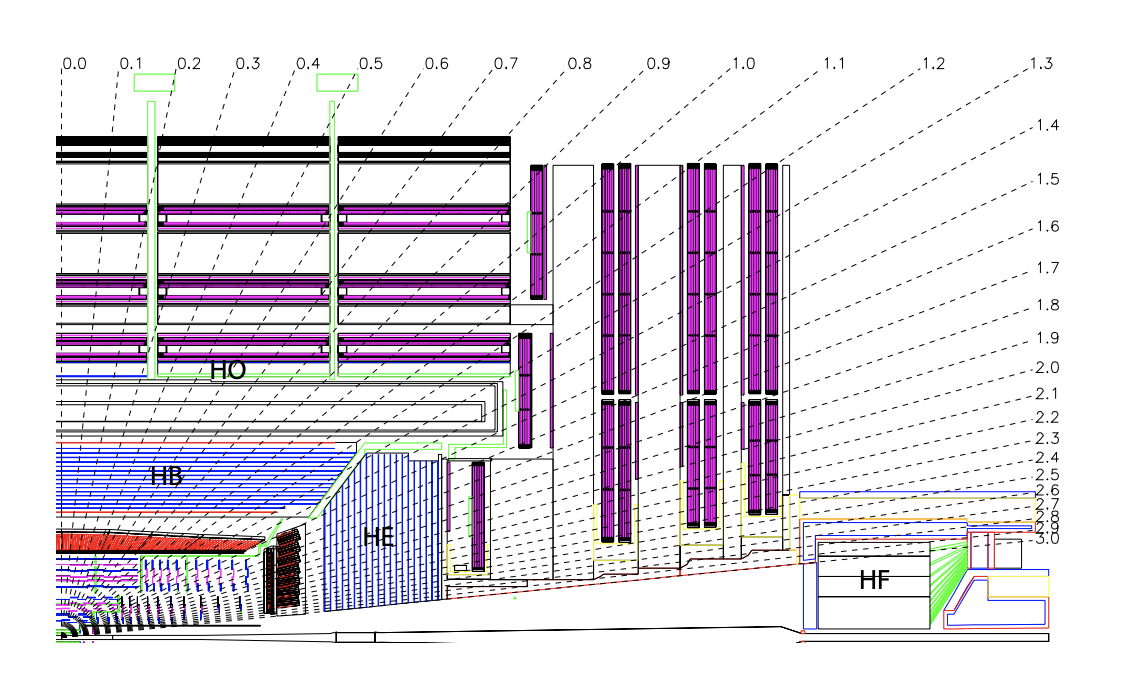
\includegraphics[width=15cm]{hcal_layout.png}
    \end{minipage}
    \caption{Longitudinal view of the CMS detector showing the locations of the hadron barrel (HB), endcap (HE), outer (HO) 
    and forward (HF) calorimeters ~\cite{cms:cms_experiment}.}
    \label{fig:hcal_layout}
\end{figure}

\subsection{Muon System}

Muon detection is of great importance to the CMS, since it is a powerful tool for recognizing signatures of interesting physics processes. Muons also have the
potential to be reconstructed with a larger resolution since they are less affected by radiative losses in the tracker material, compared to electrons. 

The muon system is installed in the psuedo-rapidity range of $|\eta| < 2.4$, consisting of drift tubes (DTs), cathode strip chambers (CSCs) and 
resistive plate chambers (RPCs). The DTs are placed in the barrel and cover the $|\eta| < 1.2$ range, where the particle rate and the local 
magnetic fill strength are low. CSCs, due to their fast response time, fine segmentation, and radiation resistance, are used in the endcap, covering
$0.9 < |\eta| < 2.4$. RPCs are inserted into both barrel and endcaps to provide redundant trigger system with a time resolution of 1 ns, 
which is much shorter than the bunch crossing interval of 25 ns.

\subsection{Trigger System}
\label{subsec:trigger_system}

With a proton-proton bunch crossing interval of $25$ ns, collecting and saving all collision events at a rate of $400$ MHz in unsustainable, 
due to limitations in both storage space and data transfer rates. 
Storing all the events at this rate is also unnecessary, since interesting events with high-energy physics objects occur at a much
lower rate.

To select the events of interest and reduce the rate of data being saved, a two-tiered trigger system is being used in the CMS experiment. The first-level
trigger (L1), is composed of custom hardware processors, which uses event information from the calorimeters and the muon system to select events at a rate
of 100 kHz within a fixed latency of about 4 $\mu s$ \cite{cms:l1_paper}. The second level, known as the high-level trigger (HLT), consists of processors 
running a version of the full event reconstruction software optimized for fast processing, and reduces the event rate to around 1 kHz before data storage 
\cite{cms:hlt_paper}. 

% The following subsection will go into further details about the HLT system and the related upgrade work done which is relevant for this thesis.

% \subsubsection{High-level Trigger System}

% High-level trigger (HLT) in CMS is the last step of event selection before accepted events are saved for storage. The event selection at HLT is done by reconstructing
% physics objects within the event, such as electrons, muons, jets and missing transverse momentum (the definition of these objects are provided in Sec.~\ref{sec:objects}).
% During this reconstruction, information from all detectors are used to identify different types of particles. Several identification
% criteria are applied on these reconstructed physics objects to select events of potential interest.

% The event selection in the HLT is structured around the concept of a \textit{HLT path}. Each HLT path is a sequence of processes running in a pre-defined order, which
% reconstructs physics objects and applies selections on them. At the end of processing, each HLT path will return a $0/1$ decision indicating whether the event is accepted
% for storage or not. Typically, each HLT path is implemented as a sequence of processing steps with increasing complexity. As an example, selections relying only on calorimeter
% information are applied first to reduce the event rate, and then the more CPU-expensive tracking reconstruction is performed to apply further selections on physics objects.
% A detailed summary of how each object is reconstructed is given in~\cite{cms:hlt_paper}.     

% Typically, every HLT path targets the identification of a single type of physics object (e.g. jets), and applies a filter on that object to decide whether to accept or reject
% the event.
